Temporal interoperability implies that multiple, possibly heterogeneous media
components may easily be combined into a single, consistently timed media
experience~\cite{temporalcomposition}. We argue that temporal interoperability must be promoted as a
principal feature of the Web, and finding the right approach to media
synchronization is key to achieving this. In this section we distinguish two
basic approaches, \emph{internal timing} and \emph{external timing}, and
explain why external timing is better suited as a basis for temporal
interoperability. Note that extenal timing is provided by motions\footnote{mediated by timing objects} 
according to the
motion model.

\begin{figure}[h]
%\sidecaption
\centering
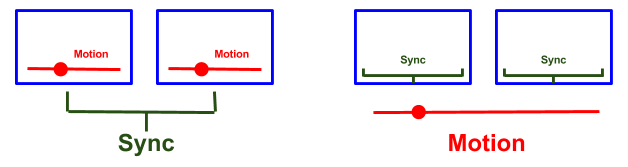
\includegraphics[scale=.4]{fig/internal-external.png}
\caption{
	Blue rectangles represent media components, red symbols represent motion, and green symbols represent the process of media synchronization. To the left: internal timing and external media synchronization. To the right: external timing and internal media synchronization.
}
\label{fig:internalexternal}
\end{figure}


\subsection{Internal timing}

Internal timing is the most familiar one, where media components are typically
media players or frameworks internalizing aspects of timing and control.
Synchronizing such media components is an external process, utilizing the
control primitives provided by each component.

Internal timing means that media components implement timed operations
internally, based on the system clock or some other (hardware) timer and state
representing motion. Timed operations may also be affected by other internal
factors, such as the buffering of timed data, time consumption in processing,
or delays in UI pipelines. The outside world is typically given access to the
internal motion of the media component via interactive elements in the UI, or
programmatically through control primitives defined in the component API. For
example, the HTML5 media element allows media playback to be requested by
clicking the play button or invoking the play method. The media element then
organizes media playback in its own time, subject to delays in initialisation
procedures, buffering, decoding and AV-subsystems.

\subsection {External timing}

External timing is the opposite approach, where media components consider
themselves parts of a bigger experience. Such media components are explicitly
designed to take direction from an external motion, and always do their best
to synchronize their own behavior accordingly. If multiple media components
are connected to the same external motion, synchronized behavior across media
components follows by implication. In this approach, media synchronization is
redefined as an internal challenge, to be addressed by each media component
independently.


\runinhead{Media control:}

The external timing approach implies that control over the media component is
exercised indirectly, by manipulating the external motion instead of the media
component. For instance, if the external motion is paused or time-shifted, the
media component must react accordingly. Appropriate controls for the media
component may still be exposed through the UI or API of the component.
However, such control requests must be routed to the external motion. This
ensures that control applies to all media components connected to the same
external motion. It also ensures that media components may process control
requests without regard to the origin of the request. Importantly, media
components directed by external motions may still make use of an internal
clock. Importantly though, the external motion takes precedence, so deviations
must be compensated for by adjusting the internal clock.

\runinhead{Precision:}

Precision is a key ambition in media synchronization. With internal timing,
synchronization with other media is performed using the control primitives
that each media component defines. In the Web environment, such control
primitives have typically not been designed with precise timing in mind  (see
Sect.~\ref{sec:web-html}).  This makes high quality synchronization hard to
achieve. In this model media synchronization generally gets more difficult as
the number of components increases. Heterogeneity in media types and control
interfaces complicate matters further. For precise synchronization, external
timing appears to be a better approach. Media synchronization is solved
internally in media components, where it can be implemented with unrestricted
access to the internal state and capabilities of the component. Furthermore,
the synchronization task is shifted from external application developers to
the author of the media component. This makes sense, as the author likely has
better understanding of how the media component works. It also ensures that
the problem may be solved once, instead of repeatedly by different application
developers.


\runinhead{Buffering:}

Another distinctive feature of the external motion approach is that motion is
not sensitive to the internal state (e.g. data availability) of any media
component. For instance, external motion might describe playback while a
particular media component still lacks data. In the external motion approach,
media components must always align themselves with the external motion, to the
best of their abilities. For example, media components may adapt by buffering
data further ahead, changing to a different data source (e.g. lower bitrate)
or even changing to a different presentation mode (e.g audio only). This way,
playback may continue undisturbed and media components join in as soon as they
are able to. This is particularly important in multi-device scenarios, where a
single device with limited bandwidth might otherwise hold back the entire
presentation. On the other hand, if the readiness of a particular media
component is indeed essential to the experience, this may be solved in
application code, by pausing and resuming the external motion.


\runinhead{Master-Slave:}

Asymmetric master slave synchronization is a common pattern in media
synchronization. The pattern implies that internal motion of a master media
component is used as external motion for slave media components. However, with
multiple media components all but one must be a slave. In the external timing
approach all media components are slaves, and the external motion itself is
the master. This avoids added complexities of the master-slave  pattern, and
provides a symmetric model where each media component may request control via
the external motion. On the other hand, if asymmetry is indeed appropriate for
a given application, this may easily be emulated. For instance, applications
may ensure that only one specific media component may issue control requests
to the external motion.

\runinhead{Live and on-demand:}

Solutions for live media often target minimized transport latency for real-time 
presentation. In other words, the internal motion of live media
components is tied to data arrival. This may be problematic in some
applications, as differences in transport latency imply that media components
will be out of sync. For example, live Web-based streaming solutions may be
seconds apart, even on the same network. Timing issues with live media is even
more evident in rich media productions involving multiple live feeds with very
different production chains and transport mechanisms. The external timing
approach provides the control and flexibility needed for applications to deal
with these realities in appropriate ways. With an external motion representing
the official live motion, multiple live media sources may be presented in a
time-consistent way across components and screens. Such a live motion could be
selected to cover at least a majority of viewers. Furthermore, inability to
follow the official live motion would be detected by media components
internally, potentially triggering application specific reactions. For
instance, the viewer could be prompted to switch to a private, slightly time-shifted 
motion suitable for his or her specific environment.

